% `template.tex', a bare-bones example employing the AIAA class.
%
% For a more advanced example that makes use of several third-party
% LaTeX packages, see `advanced_example.tex', but please read the
% Known Problems section of the users manual first.
%
% Typical processing for PostScript (PS) output:
%
%  latex template
%  latex template   (repeat as needed to resolve references)
%
%  xdvi template    (onscreen draft display)
%  dvips template   (postscript)
%  gv template.ps   (onscreen display)
%  lpr template.ps  (hardcopy)
%
% With the above, only Encapsulated PostScript (EPS) images can be used.
%
% Typical processing for Portable Document Format (PDF) output:
%
%  pdflatex template
%  pdflatex template      (repeat as needed to resolve references)
%
%  acroread template.pdf  (onscreen display)
%
% If you have EPS figures, you will need to use the epstopdf script
% to convert them to PDF because PDF is a limmited subset of EPS.
% pdflatex accepts a variety of other image formats such as JPG, TIF,
% PNG, and so forth -- check the documentation for your version.
%
% If you do *not* specify suffixes when using the graphicx package's
% \includegraphics command, latex and pdflatex will automatically select
% the appropriate figure format from those available.  This allows you
% to produce PS and PDF output from the same LaTeX source file.
%
% To generate a large format (e.g., 11"x17") PostScript copy for editing
% purposes, use
%
%  dvips -x 1467 -O -0.65in,0.85in -t tabloid template
%
% For further details and support, read the Users Manual, aiaa.pdf.


% Try to reduce the number of latex support calls from people who
% don't read the included documentation.
%


\typeout{}\typeout{If latex fails to find aiaa-tc, read the README file!}
%


\documentclass[]{aiaa-tc}% insert '[draft]' option to show overfull boxes
\usepackage{float}
\usepackage{epstopdf}
\usepackage{amsmath}
\usepackage[table,xcdraw]{xcolor}

\title{Attitude Estimation}

\author{
	Johnathan Clouse%
	\thanks{Graduate Student, Aerospace Engineering Sciences, 1111 Engineering Drive, Boulder, CO, 80309-0429}\\
	{\normalsize\itshape
		University of Colorado, Boulder, CO, 80309-0429, USA}
}

% Define commands to assure consistent treatment throughout document
\newcommand{\eqnref}[1]{(\ref{#1})}
\newcommand{\class}[1]{\texttt{#1}}
\newcommand{\package}[1]{\texttt{#1}}
\newcommand{\file}[1]{\texttt{#1}}
\newcommand{\BibTeX}{\textsc{Bib}\TeX}

\usepackage[euler]{textgreek}
\usepackage[colorlinks=true]{hyperref}
\hypersetup{urlcolor=cyan}

\usepackage{listings}
\usepackage{color} %red, green, blue, yellow, cyan, magenta, black, white
\definecolor{mygreen}{RGB}{28,172,0} % color values Red, Green, Blue
\definecolor{mylilas}{RGB}{170,55,241}

\usepackage{tablefootnote}
\usepackage{graphicx}
\usepackage{amsmath}
\usepackage{bm}
\usepackage{subfigure}
%\usepackage{subcaption}

\definecolor{mylilas}{RGB}{170,55,241}

% See p.105 of "TeX Unbound" for suggested values.
% See pp. 199-200 of Lamport's "LaTeX" book for details.
%   General parameters, for ALL pages:
\renewcommand{\topfraction}{0.9}	% max fraction of floats at top
\renewcommand{\bottomfraction}{0.8}	% max fraction of floats at bottom
%   Parameters for TEXT pages (not float pages):
\setcounter{topnumber}{2}
\setcounter{bottomnumber}{2}
\setcounter{totalnumber}{4}     % 2 may work better
\setcounter{dbltopnumber}{2}    % for 2-column pages
\renewcommand{\dbltopfraction}{0.9}	% fit big float above 2-col. text
\renewcommand{\textfraction}{0.07}	% allow minimal text w. figs
%   Parameters for FLOAT pages (not text pages):
\renewcommand{\floatpagefraction}{0.7}	% require fuller float pages
% N.B.: floatpagefraction MUST be less than topfraction !!
\renewcommand{\dblfloatpagefraction}{0.7}	% require
    \makeatletter
    \renewcommand\l@section{\@dottedtocline{2}{1.5em}{3em}}
    \makeatother
    
\begin{document}
	

	
	\maketitle
	
	\begin{abstract}
		\noindent 
		
	\end{abstract}
	
	\newpage
	
	\tableofcontents
	
	\newpage

	\section{Introduction}
Estimation of spacecraft attitude can provide solutions needed for control inputs. Many spacecraft have payloads that must be pointed in a specified direction to perform their function; attitude knowledge is the first step of that process. 

	\vspace{5 mm}

Attitude can be represented in several ways. The most fundamental representation is a 3x3 direction cosine matrix, which can transform a vector from one frame to another. However, it has a total of nine elements. Euler angles can represent the same orientation in three elements. But, like all three-element representations, singularities can occur at certain rotations. Quaternions are representations that are universally non-singular, but they have four constrained elements.

	\vspace{5 mm}

This paper will identify the dynamics for a gravity gradient microsatellite. It will then detail two methods of attitude determination: an EKF estimating the Euler yaw-pitch-roll angles, and the Multiplicative EKF.
	
	\section{Attitude Dynamics}
The rotational equations of motion are given by Equation \ref{eqn:EOM}, where $I_{xx}$ is the mass-moment of inertia about a principle axis and $\omega$ is the body rate about that axis.  
	\begin{equation}
		\begin{matrix}
		I_{11}\dot{\omega_1}=-(I_{33}-I_{22})\omega_2\omega_3+T_1\\ 
		I_{22}\dot{\omega_2}=-(I_{11}-I_{33})\omega_3\omega_1+T_2\\ 
		I_{33}\dot{\omega_3}=-(I_{22}-I_{11})\omega_1\omega_2+T_3
		\end{matrix}
		\label{eqn:EOM}
	\end{equation}

The kinematic equation for a yaw-pitch-roll ($\psi$, $\theta$, $\phi$) representation is shown in Equation\ref{eqn:diffEqEuler}\cite{SchaubJunkins}. It is useful due to how the body rate vector $\boldsymbol{\omega}$ is separated, allowing for a change in Euler-angle representation if a singularity is being approached.
	\begin{equation}		
		\begin{pmatrix}
		\dot{\psi}\\ 
		\dot{\theta}\\ 
		\dot{\phi}
		\end{pmatrix} = 
		\frac{1}{\cos \theta}\begin{bmatrix}
		0 & \sin\phi & \cos\phi \\ 
		0 & \cos\phi\cos\theta & -\sin\phi\cos\theta\\ 
		\cos \theta & \sin\phi\sin\theta & \cos\phi\sin\theta
		\end{bmatrix}
		\begin{pmatrix}
		\omega_1\\ 
		\omega_2\\ 
		\omega_3
		\end{pmatrix}=
		B(\psi,\theta\phi)\boldsymbol{\omega}
		\label{eqn:diffEqEuler}
	\end{equation}

Gravity-gradient torque is given by Equation \ref{eqn:GGTorque}\cite{SchaubJunkins}:

	\begin{equation}
		\vec{T}_{grav} = \frac{3\mu}{R^5}\begin{pmatrix}
		R_2R_3(I_{33}-I_{22})\\ 
		R_1R_3(I_{11}-I_{33})\\ 
		R_1R_2(I_{22}-I_{11})
		\end{pmatrix}
		\label{eqn:GGTorque}
	\end{equation}

\noindent where $mu$ is Earth's gravitational parameter and $R$ is the vector from the center of the Earth to the spacecraft center of mass, expressed in the body frame. $R$ is obtained through inertial knowledge (either ephemeris or estimated) and rotated by the DCM in Equation \ref{eqn:DCM_Euler}.
	\begin{equation}
		DCM_{YPR} = \begin{bmatrix}
		\cos\theta\cos\psi & \cos\theta\sin\psi & -\sin\theta\\ 
		\sin\phi\sin\theta\cos\psi -\cos\phi\sin\psi& \sin\phi\sin\theta\sin\psi+\cos\phi\cos\psi & \sin\phi\cos\theta\\ 
		\cos\phi\sin\theta\cos\psi+\sin\phi\sin\psi & \cos\phi\sin\theta\sin\psi-\sin\phi\cos\psi & cos\phi\cos\theta
		\end{bmatrix}
		\label{eqn:DCM_Euler}
	\end{equation}

Combining the Equations \ref{eqn:diffEqEuler}, \ref{eqn:GGTorque}, and \ref{eqn:DCM_Euler} lead to the kinematic Equation \ref{eqn:EulerGGDiffEq}\cite{SchaubJunkins}:
	\begin{equation}
		\begin{pmatrix}
		\dot{\psi}\\ 
		\dot{\theta}\\ 
		\dot{\phi}
		\end{pmatrix} = 
		B(\psi,\theta\phi)\boldsymbol{\omega}-\frac{\Omega}{\cos\theta}\begin{pmatrix}
		\sin\theta\sin\psi\\ 
		-\cos\theta\cos\psi\\ 
		-\sin\psi
		\end{pmatrix}
		\label{eqn:EulerGGDiffEq}
	\end{equation}

Equation \ref{eqn:EulerGGDiffEq} are the kinematics of a yaw-pitch-roll angle representation of attitude of the spacecraft body with respect to the Local Vertical, Local Horizontal (LVLH) frame. The LVLH frame in this paper is one where the vertical axis is anti-orbit-radial, and the cross-axis is anti-orbit-normal. This is the LVLH definition used by Johnson Space Center.

	\section{Simulation}

A microsatellite in low Earth orbit was simulated to provide data to be filtered. The simulated state was comprised of Earth-inertial position and velocity, the inertial-to-body quaternion, and the inertial rates expressed in the body frame. Position and velocity were propagated with a two-body point-mass model, while attitude was propagated with gravity gradient torque using Equations \ref{eqn:EOM} and \ref{eqn:GGTorque}. Table \ref{table:SimParams} lists the parameter values that were used in the simulation.

% Please add the following required packages to your document preamble:
% \usepackage[table,xcdraw]{xcolor}
% If you use beamer only pass "xcolor=table" option, i.e. \documentclass[xcolor=table]{beamer}
\begin{table}[H]
\centering
\caption{Simulation Parameters}
\label{table:SimParams}
\begin{tabular}{|l|l|}
\rowcolor[HTML]{C0C0C0} 
\textbf{Parameter}                                                                    & \textbf{Value} \\ \hline
Orbit Semi-major axis                                                                 & 6678 km        \\ \hline
Orbit Eccentricity                                                                    & 0              \\ \hline
Orbit Inclination                                                                     & 23$^\circ$             \\ \hline
Orbit Arg of Periapse                                                                 & 0$^\circ$              \\ \hline
\begin{tabular}[c]{@{}l@{}}Orbit Right Ascention\\ of the Ascending Node\end{tabular} & 0$^\circ$              \\ \hline
Initial true anomaly                                                                  & 0$^\circ$              \\ \hline
Spacecraft Mass                                                                       & 50 kg          \\ \hline
Spacecraft Length                                                                     & 0.5 m          \\ \hline
Spacecraft Width                                                                      & 0.316 m             \\ \hline
$\mu_{Earth}$                                                                      & 3.986e5 km            \\ \hline
\end{tabular}
\end{table}

The results of the simulation are shown in Figure \ref{fig:SimResults} below.
	\begin{figure}[H]
		\centering
		\subfigure[Euler angles wrt LVLH]{
			\includegraphics[width = 12cm]{../Figures/sim_angles.eps}
		}
		\subfigure[Body Rates]{
			\includegraphics[width = 12cm]{../Figures/sim_rates.eps}
		}
		\caption{Simulation results }
		\label{fig:SimResults}
	\end{figure}	

As expected, the gravity-gradient torque produced an oscillatory motion about the pitch and roll axes. The body yaw rate stays at zero due to the spacecraft symmetry, but the yaw in the euler representation is non-zero because it's a component of the attitude representation.

	\vspace{5 mm}

To simulate measurements, the rates were sampled at 1 Hz with noise of mean 0 rad/s and standard deviation of 1e-6 rad/s. Direct Euler-angle measurements were also modeled, possibly from a composite attitude device (sun sensor with Earth sensor) or a (very coarse, as explained) star tracker. Noise was added with the model with mean 0$^\circ$ and standard deviation of 0.165$^\circ$, applied about each Euler angle rotation.

	\section{Filtering the Euler Representation}

An Extended Kalman Filter was developed for estimating the Euler-angle representation of attitude from LVLH. The state being estimated was
\begin{equation}
X=\begin{pmatrix}
\psi\\ 
\theta\\ 
\phi\\ 
\boldsymbol{\omega}
\end{pmatrix}
\label{eqn:stateEuler}
\end{equation}

The dynamic model was linearized about $X=0$, which is the equilibrium state for a gravity-gradient satellite. The direct attitude and rate measurements lead to simple measurement sensitivity matrices. For angles only:
\begin{equation}
H=\begin{bmatrix}
I_{3\times 3} & 0_{3\times 3}
\end{bmatrix}
\label{eqn:H_Euler}
\end{equation}

\noindent For body rates only:
\begin{equation}
H=\begin{bmatrix}
0_{3\times 3} & I_{3\times 3}
\end{bmatrix}
\end{equation}

\noindent For both measurement types:
\begin{equation}
H=
I_{6\times 6}
\label{eqn:H_Euler}
\end{equation}

\noindent All of these measurement sets make the system observable.  The position and velocity states are not estimated; instead, they are propagated from ephemerides. These could be provided by ground-based observation and orbit determination.

	\vspace{5 mm}

The first filter implementation of the Euler-angle filter, a conventional Kalman filter, was run with exact \textit{a priori} state. Only rate measurements were used, and SNC variance of 1e-14 rad$^2$/s$^2$ was implemented to abate the diminishing covariance. Figure \ref{fig:ResultsEulerAPExact} shows the results.
	\begin{figure}[H]
		\centering
		\subfigure[Euler angle error]{
			\includegraphics[width = 9cm]{../Figures/CKF_apExact_AngleError.eps}
		}
		\subfigure[Body rate error]{
			\includegraphics[width = 9cm]{../Figures/CKF_apExact_RateError.eps}
		}
		\subfigure[Post-fit residuals.]{
			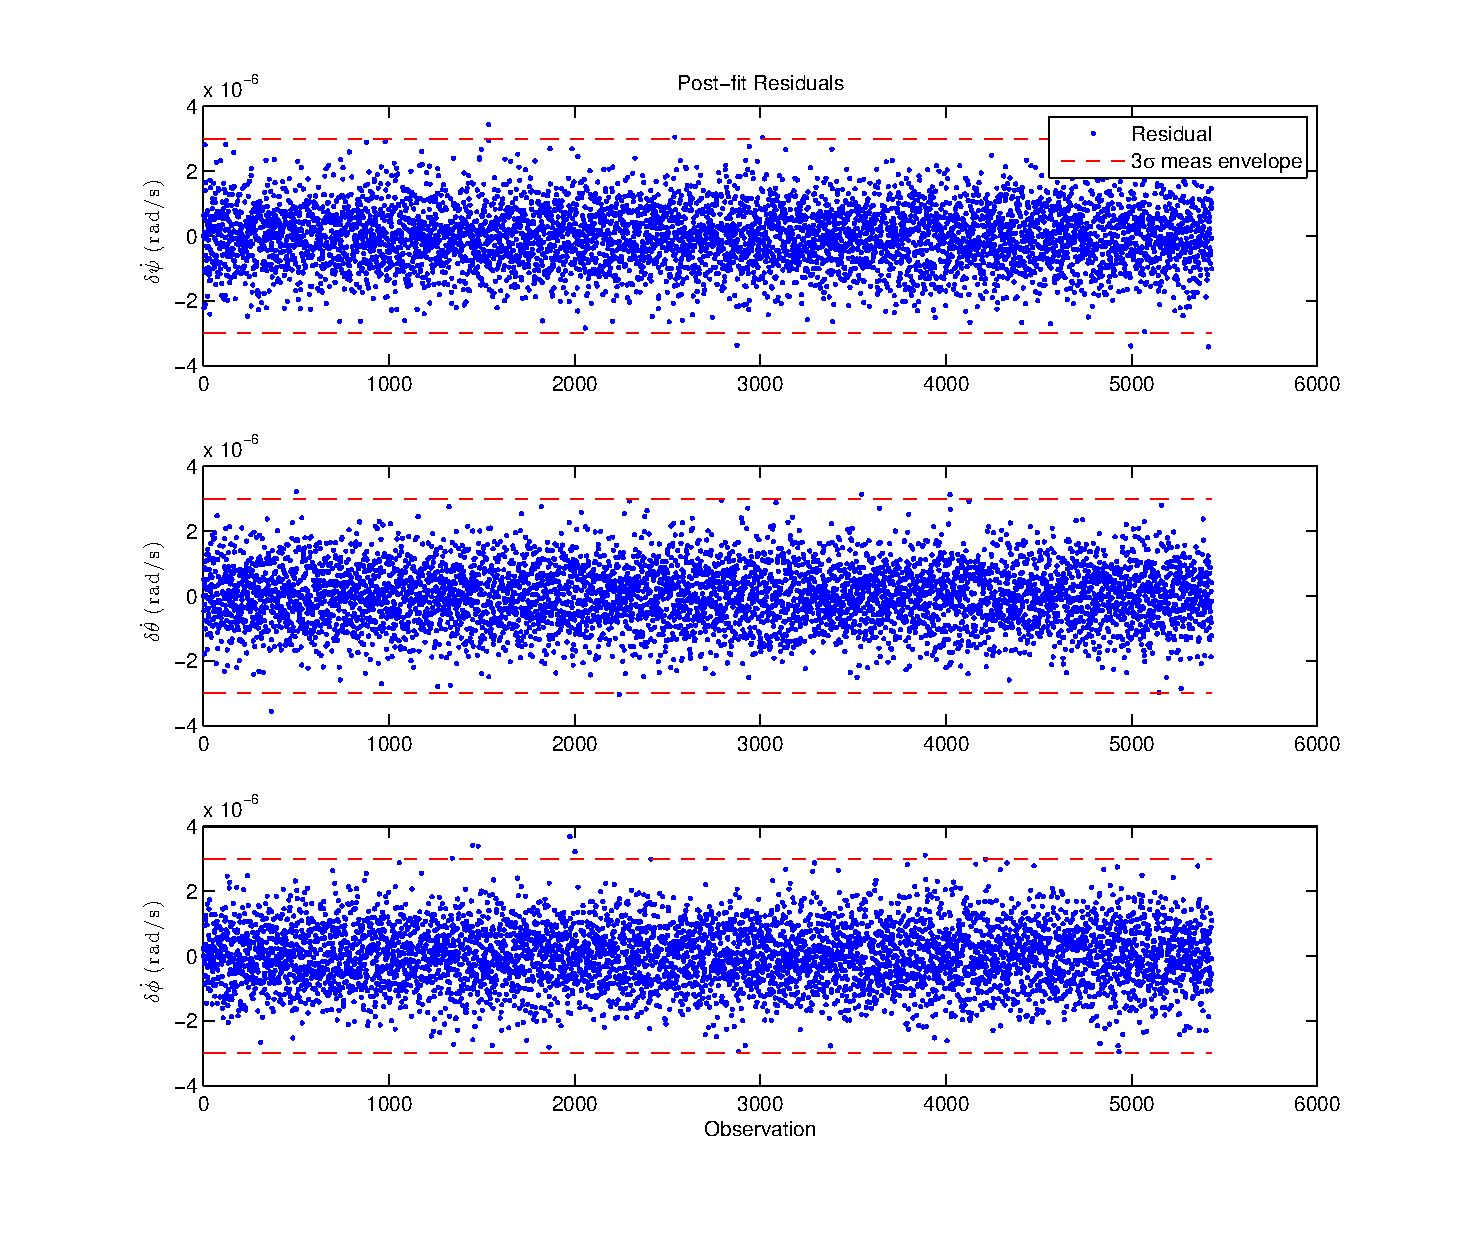
\includegraphics[width = 9cm]{../Figures/CKF_apExact_pfr.eps}
		}
		\caption{Euler-angle CKF, exact \textit{a priori} state, with rate measurements }
		\label{fig:ResultsEulerAPExact}
	\end{figure}	

As one would expect, the resulting error was small and the filter fit to the measurement noise. However, the error did not remain completely within covariance envelope. The dynamic model cannot predict change in z-axis rate at all, because the symmetry of the spacecraft forces the angular acceleration to be zero in this axis. 

	\vspace{5 mm}

In order to gain more accuracy in the yaw solution, a yaw measurement was introduced. For this gravity-gradient spacecraft, such an observation could be realistically obtained by the spacecraft being in a sun-synchronous orbit. The extended Kalman filter was used after 1000 measurements. Figure \ref{fig:ResultsEulerAPExact_yaw} shows the results.
	\begin{figure}[H]
		\centering
		\subfigure[Euler angle error]{
			\includegraphics[width = 9cm]{../Figures/EKF_Yaw_AngleError.eps}
		}
		\subfigure[Body rate error]{
			\includegraphics[width = 9cm]{../Figures/EKF_Yaw_RatesError.eps}
		}
		\subfigure[Post-fit residuals.]{
			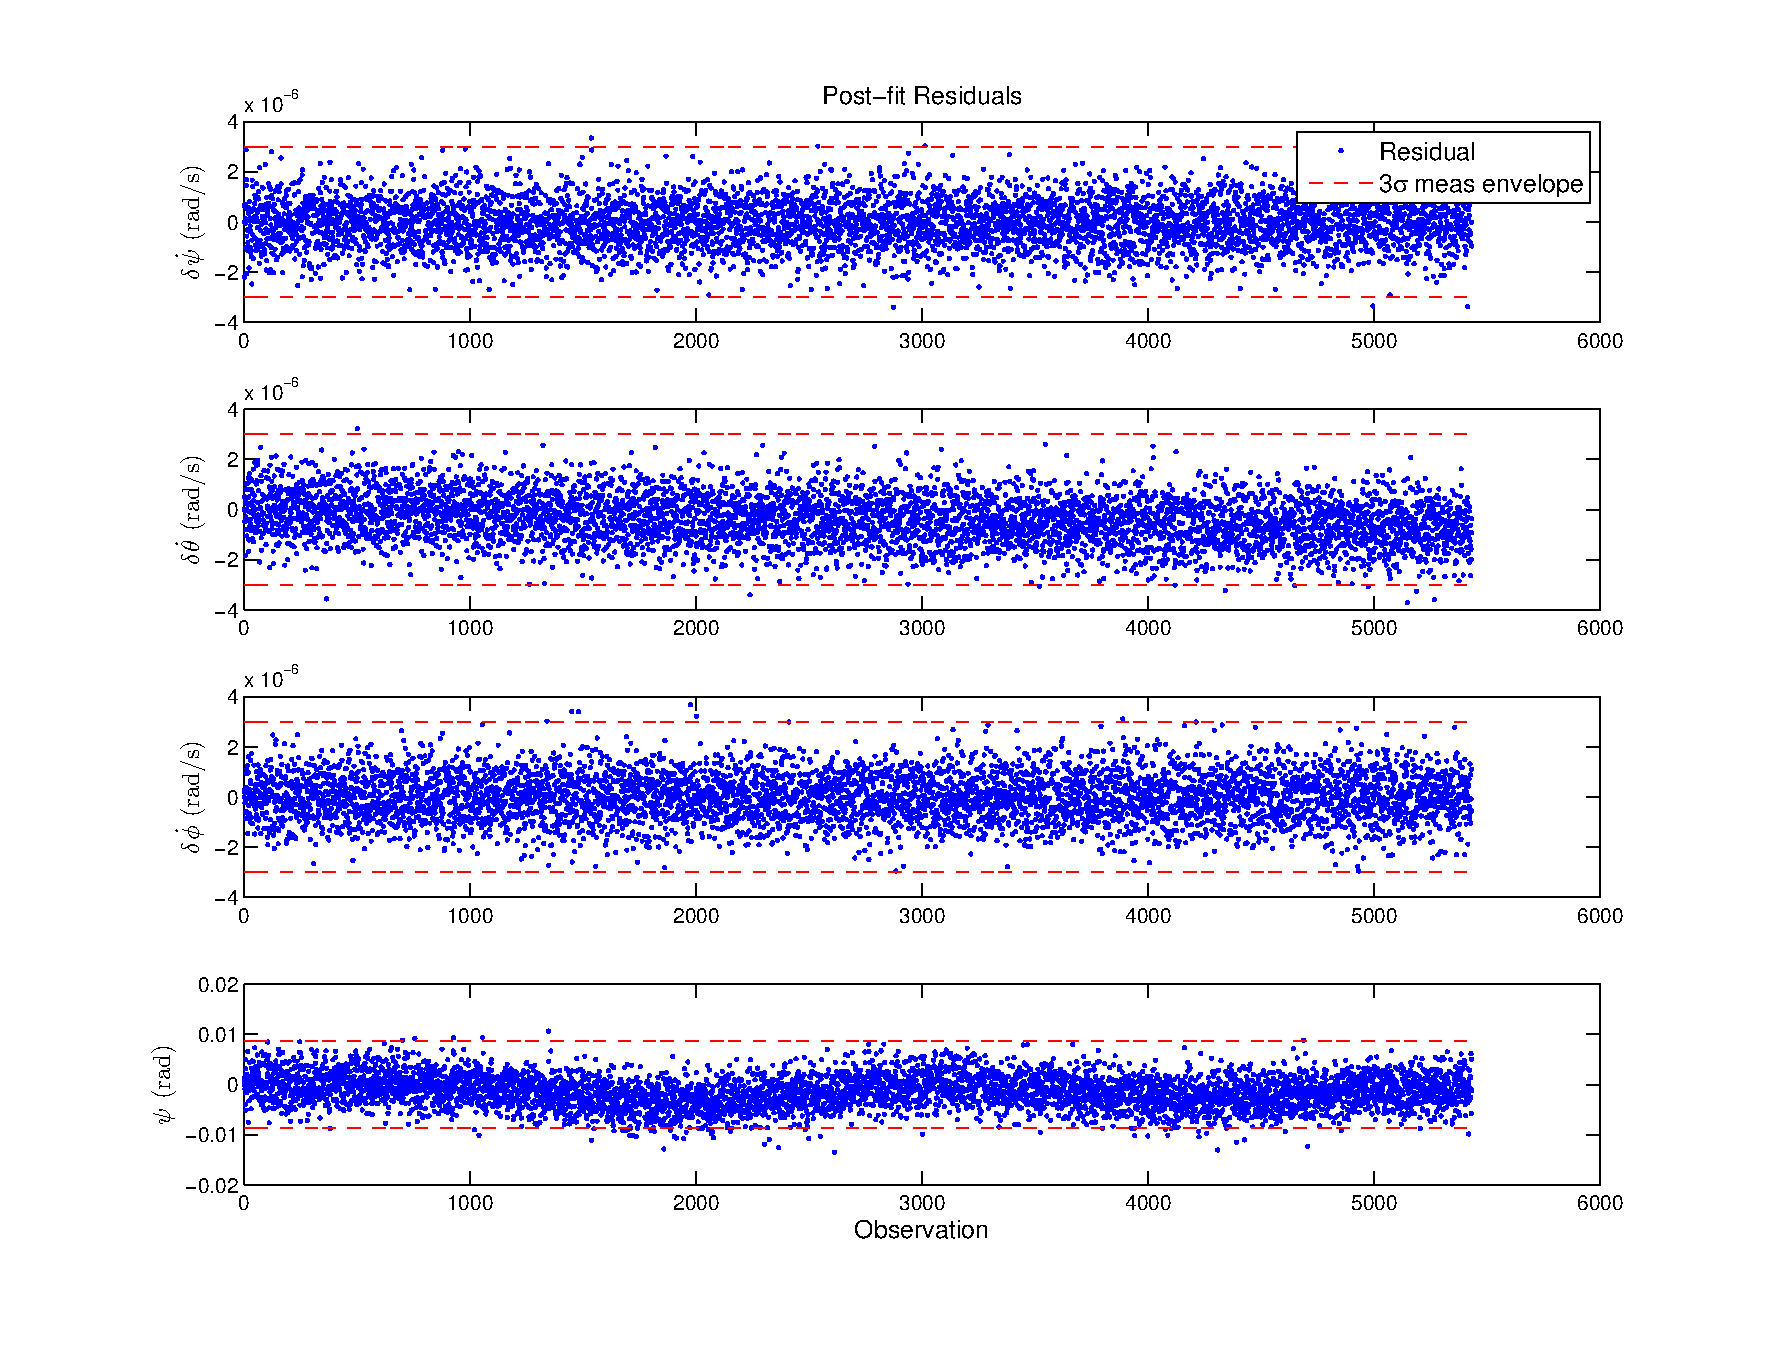
\includegraphics[width = 9cm]{../Figures/EKF_Yaw_pfr.eps}
		}
		\caption{Euler-angle EKF, exact \textit{a priori} state, with yaw measurement }
		\label{fig:ResultsEulerAPExact_yaw}
	\end{figure}	

The results are clearly poor. While yaw was initially more accurate, the pitch and roll errors stayed outside the covariance envelopes. The extended filter's state reset did not improve the estimate as desired. Further, the post-fit residuals do not match the noise.

	\vspace{5 mm}

The direct attitude measurement was incorporated without the body rate measurements. SNC was tuned to be 1e-16 rad$^2$/s$^2$ for the best post-fit residual result. Figure \ref{fig:ResultsEulerAPExact_ypr} shows the results.
	\begin{figure}[H]
		\centering
		\subfigure[Euler angle error]{
			\includegraphics[width = 9cm]{../Figures/EKF_YPR_AngleError.eps}
		}
		\subfigure[Body rate error]{
			\includegraphics[width = 9cm]{../Figures/EKF_YPR_RateError.eps}
		}
		\subfigure[Post-fit residuals.]{
			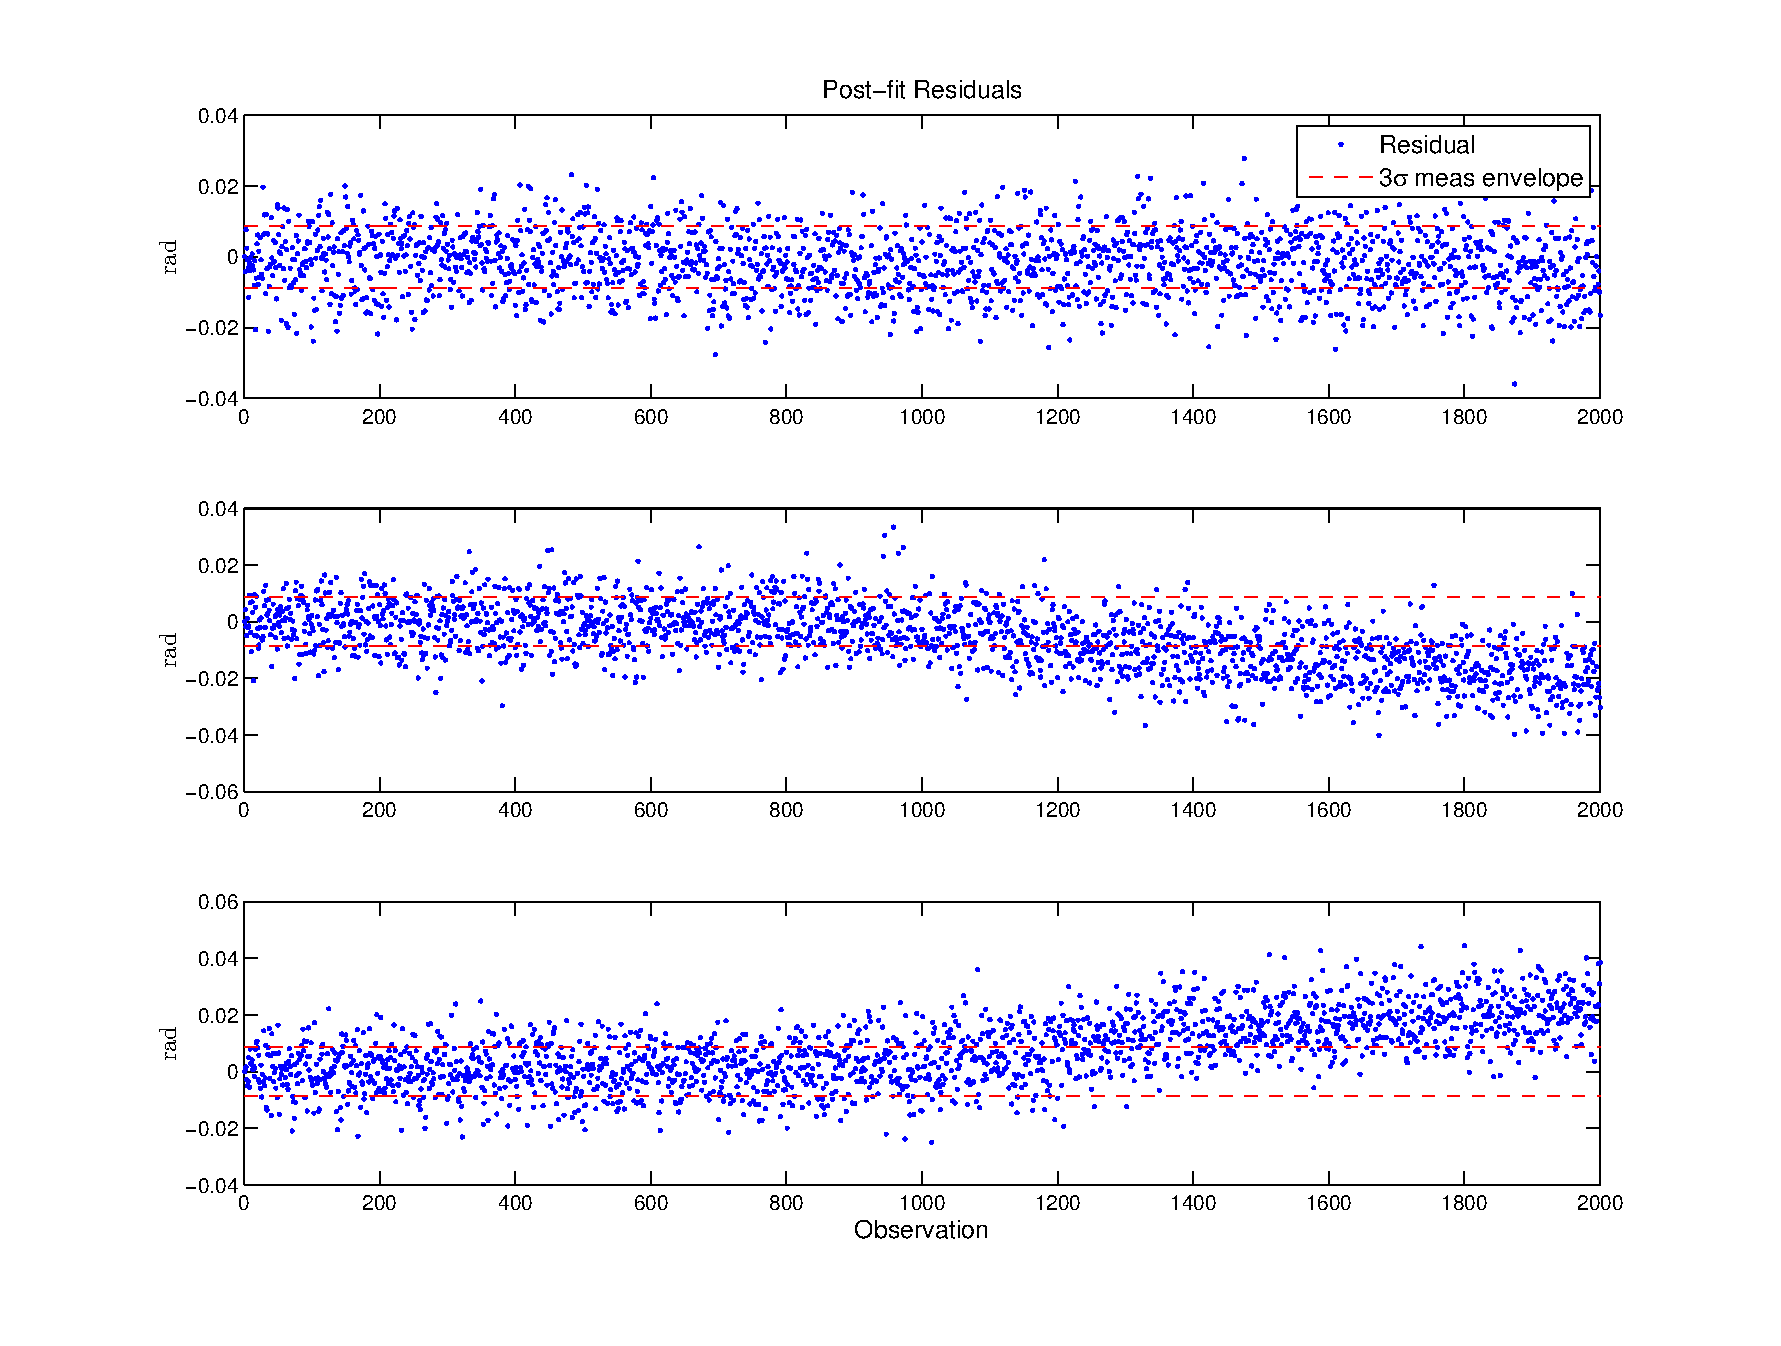
\includegraphics[width = 9cm]{../Figures/EKF_YPR_pfr.eps}
		}
		\caption{Euler-angle EKF, exact \textit{a priori} state, with yaw-pitch-roll measurements }
		\label{fig:ResultsEulerAPExact_ypr}
	\end{figure}	

The errors and residuals are, again, poor. The EKF did nothing to improve the state estimates. Pitch and roll diverged more after the EKF started.

	\vspace{5 mm}

Next, the direct attitude measurement and rate measurement were used by the filter. The exact \textit{a priori} case was successful within the covariance envelope. The \textit{a priori} state was set to $X=0$, a good estimate as any for a nominally nadir-pointing spacecraft. The EKF was also started after 200 CKF-process observations. The results are shown in Figure \ref{fig:ResultsEulerBest}.
	\begin{figure}[H]
		\centering
		\subfigure[Euler angle error]{
			\includegraphics[width = 7.75cm]{../Figures/EKF_Final_AngError.eps}
		}
		\subfigure[Body rate error]{
			\includegraphics[width = 7.75cm]{../Figures/EKF_Final_RateError.eps}
		}
		\subfigure[Euler angle post-fit residuals.]{
			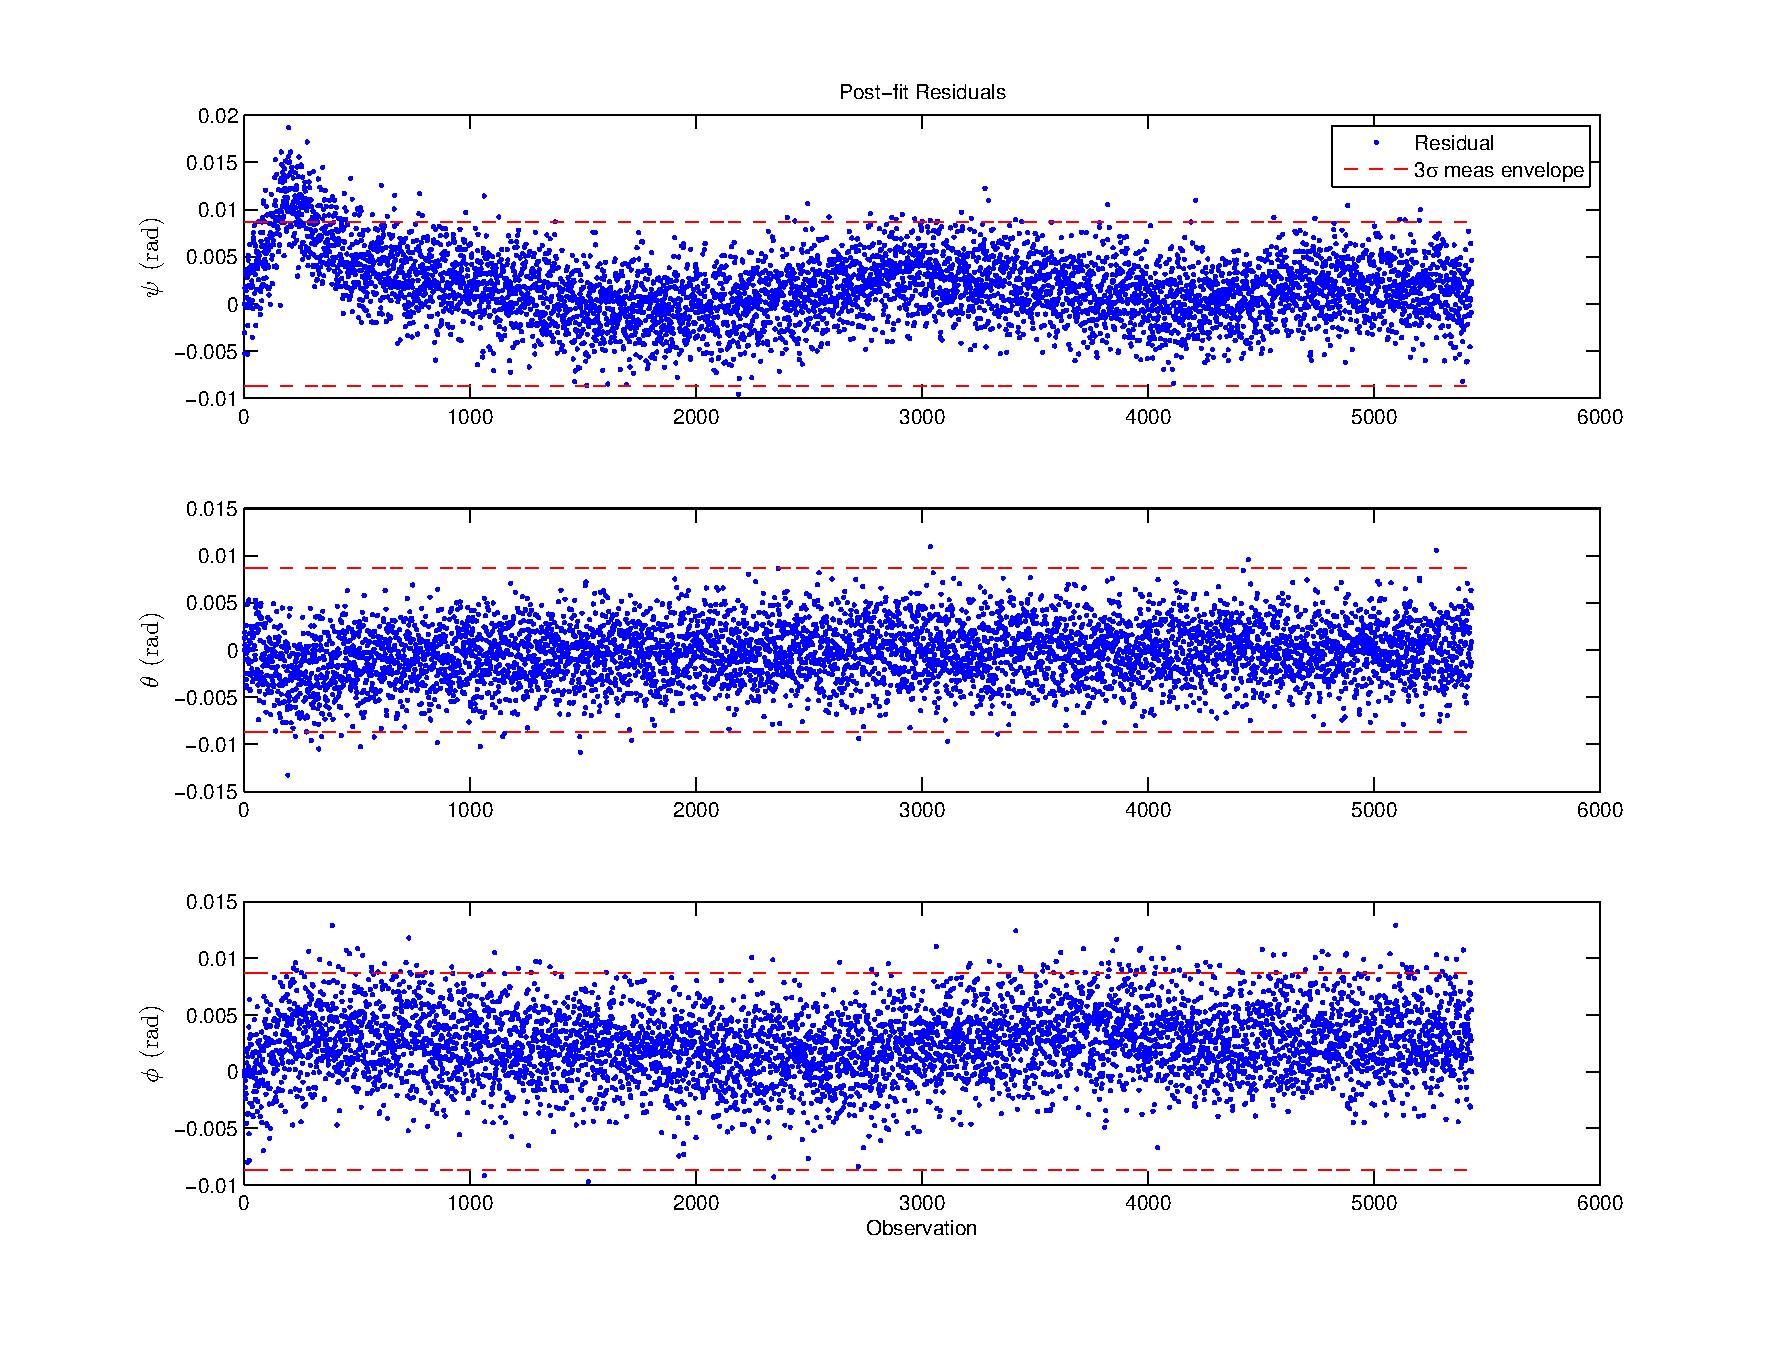
\includegraphics[width = 7.75cm]{../Figures/EKF_Final_PFR_Ang.eps}
		}
		\subfigure[Body rate post-fit residuals.]{
			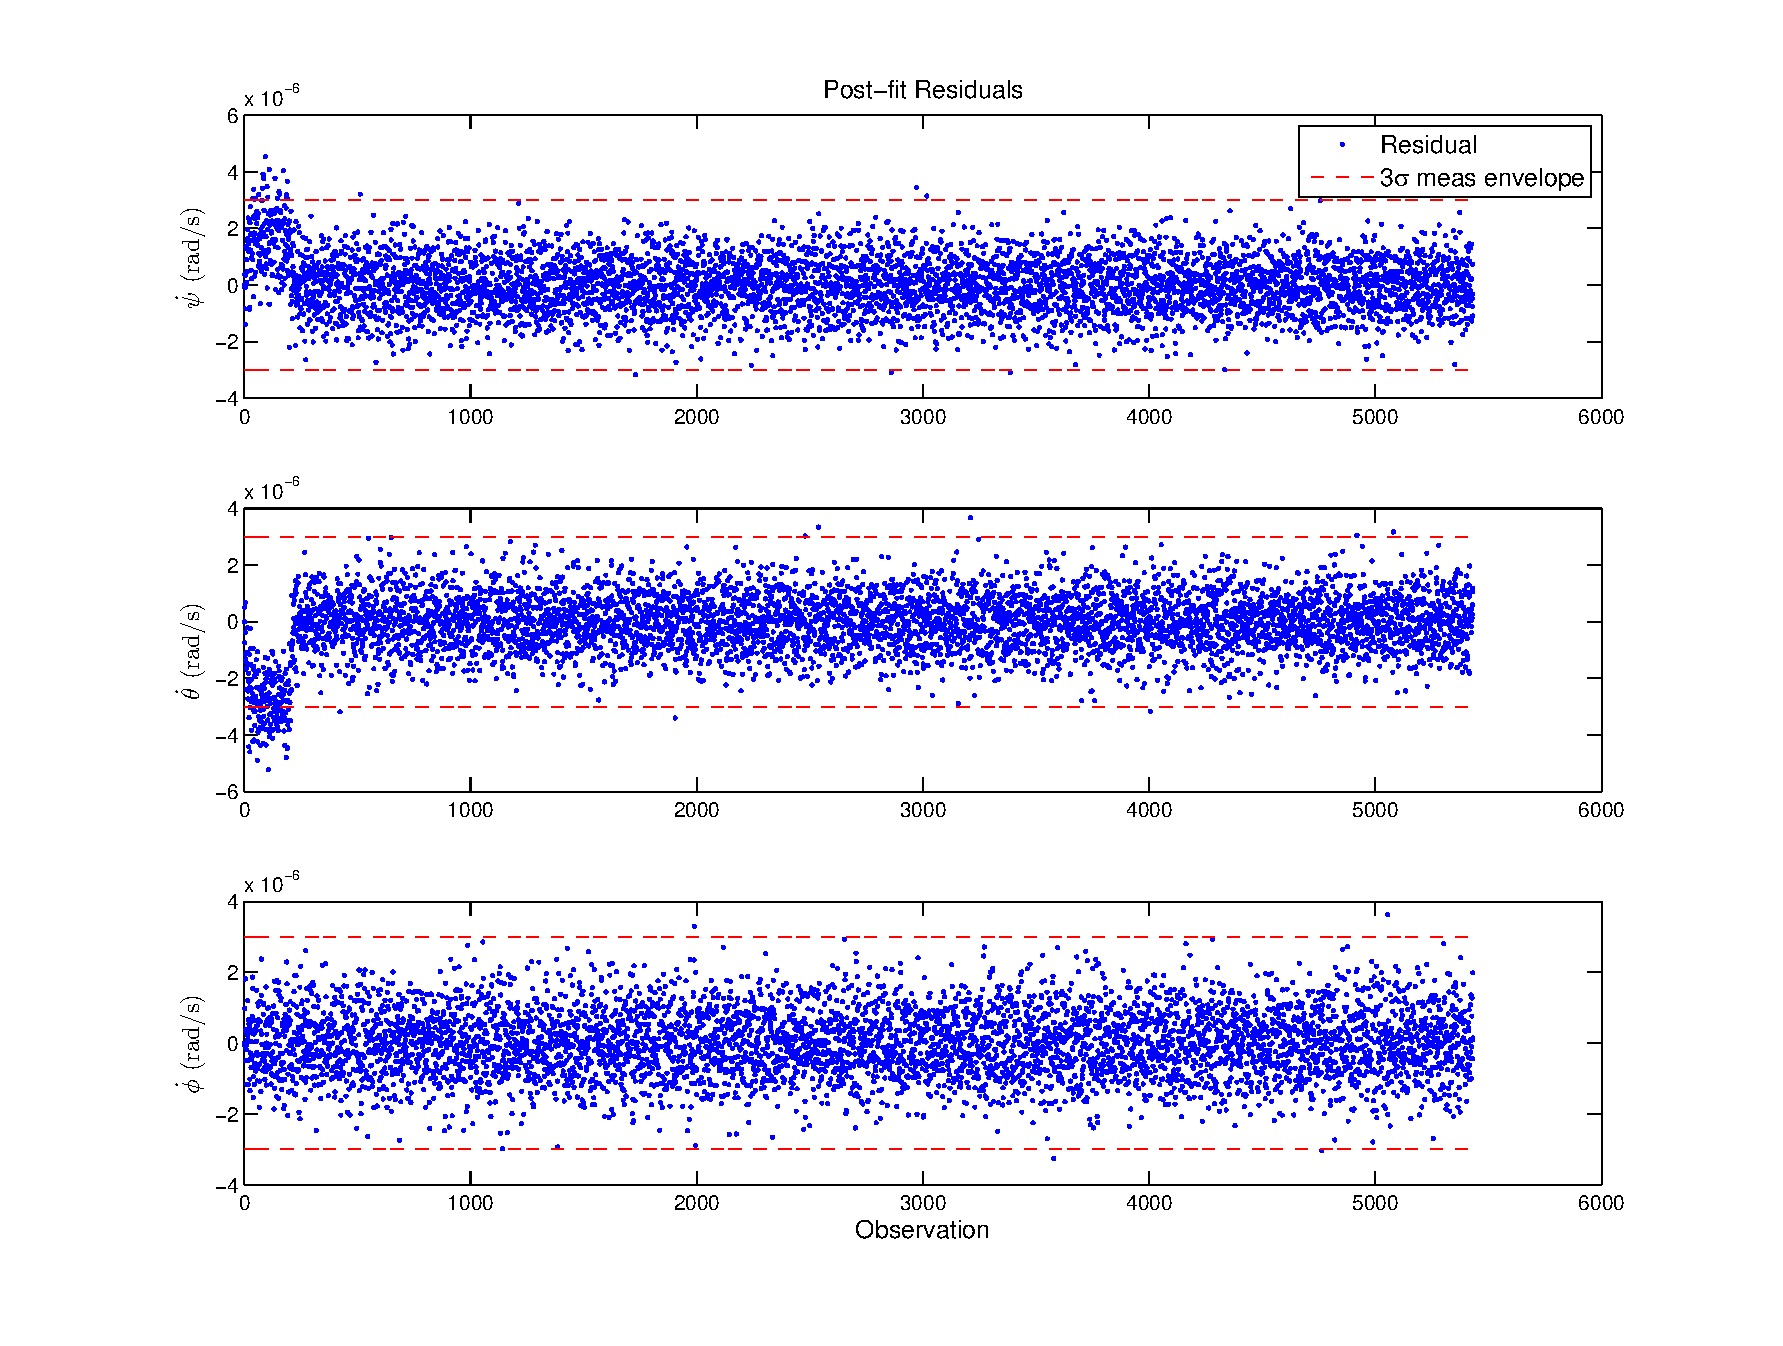
\includegraphics[width = 7.75cm]{../Figures/EKF_Final_PFR_Rates.eps}
		}
		\caption{Euler-angle EKF, \textit{a priori} state $X=0$, with yaw-pitch-roll and body rate measurements }
		\label{fig:ResultsEulerBest}
	\end{figure}	

The filter results stay close to the truth value, however, they are outside of the covariance envelope much of the time. The post-fit residuals do not match the noise well.

	\vspace{5 mm}

As a final test of the capability of this Euler-angle filter, a 10-km error was introduced in the knowledge of the orbit altitude. Figure \ref{fig:AltOff} shows how the error affected the filter estimate.
	\begin{figure}[H]
		\centering
			\includegraphics[width = 9cm]{../Figures/EKF_AltOff_AngleError.eps}

		\caption{Euler-angle EKF, exact \textit{a priori} state, with yaw-pitch-roll measurements }
		\label{fig:AltOff}
	\end{figure}	


	\section{Conclusion}




\bibliographystyle{aiaa}   % Number the references.
\bibliography{ASEN6080ProjectBib}   % Use references.bib to resolve the labels.

%    \section{Appendix B}
%This appendix contains all Matlab code used by the authors to analyize their data.
%    
%    \lstset{language=Matlab,%
%    	%basicstyle=\color{red},
%    	breaklines=true,%
%    	morekeywords={matlab2tikz},
%    	keywordstyle=\color{blue},%
%    	morekeywords=[2]{1}, keywordstyle=[2]{\color{black}},
%    	identifierstyle=\color{black},%
%    	stringstyle=\color{mylilas},
%    	commentstyle=\color{mygreen},%
%    	showstringspaces=false,%without this there will be a symbol in the places where there is a space
%    	numbers=left,%
%    	numberstyle={\tiny \color{black}},% size of the numbers
%    	numbersep=9pt, % this defines how far the numbers are from the text
%    	emph=[1]{for,end,break},emphstyle=[1]\color{red}, %some words to emphasise
%    	%emph=[2]{word1,word2}, emphstyle=[2]{style},   
%    }
    
%    \lstinputlisting{ASEN5090_ecef2azelrange.m}
%    \vspace{5mm}
%    
%    \lstinputlisting{ASEN5090_GPSvis.m}
%    \vspace{5mm}
%\lstinputlisting{HW5_rel_err.m}
%\vspace{5mm}
%\lstinputlisting{import_gps_data.m}
%\vspace{5mm}
%\lstinputlisting{datenum8601.m}
%\vspace{5mm}
%\lstinputlisting{lab_err_plots.m}
%\vspace{5mm}
	
\end{document}

% - Release $Name:  $ -
